
\documentclass{standalone}

\usepackage{pgfplots}

\usepackage{tikz,amsmath, amssymb,bm,color}

\definecolor{darkbrown}{rgb}{0.4, 0.26, 0.13}
\begin{document}
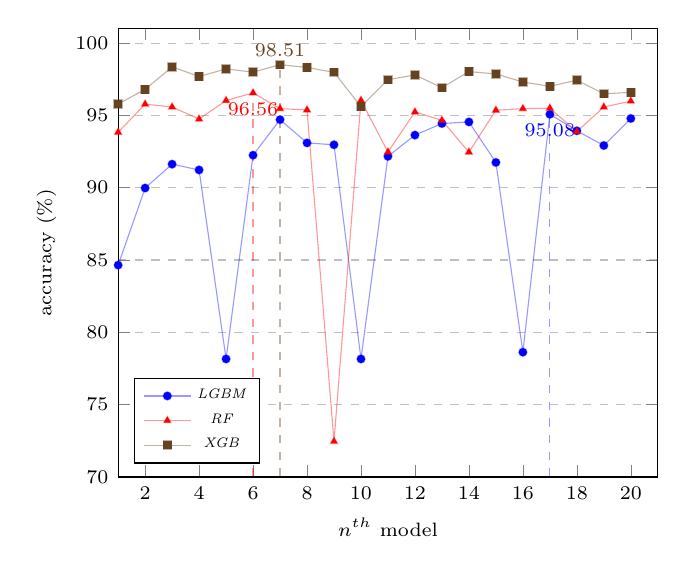
\begin{tikzpicture}
\begin{axis}[
	font = \scriptsize,
	xlabel=$n^{th}$ model,
	ylabel=accuracy (\%),
	xmin=1, xmax=21,
	ymin=70, ymax=101,
	xtick={2,4,6,8,10,12,14,16,18,20},
	ytick={70,75,80,85,90,95,100},
	ylabel near ticks,
    xlabel near ticks,
	legend pos=south west,
	legend style={mark size=2pt, font={\tiny \itshape}},
	ymajorgrids=true,
	grid style=dashed,
]
\addplot [mark=*, mark size=1.5pt, color = blue,draw opacity=0.4] coordinates {
	(1, 84.65)(2, 89.98)(3, 91.63)(4, 91.23)(5, 78.16)(6, 92.25)(7, 94.71)(8, 93.1)(9, 92.97)(10, 78.16)(11, 92.17)(12, 93.64)(13, 94.44)(14, 94.55)(15, 91.75)(16, 78.63)(17, 95.08)(18, 93.94)(19, 92.92)(20, 94.79)
};

\addplot [mark = triangle*, mark size=1.5pt, color = red, draw opacity=0.4] coordinates {
	(1, 93.84)(2, 95.78)(3, 95.58)(4, 94.75)(5, 96.03)(6, 96.56)(7, 95.47)(8, 95.38)(9, 72.46)(10, 96.04)(11, 92.47)(12, 95.24)(13, 94.66)(14, 92.46)(15, 95.36)(16, 95.47)(17, 95.5)(18, 93.88)(19, 95.58)(20, 95.99)
};


\addplot [mark = square*, mark size=1.5pt, color = darkbrown, draw opacity=0.4] coordinates {
	(1, 95.79)(2, 96.8)(3, 98.36)(4, 97.69)(5, 98.22)(6, 97.99)(7, 98.51)(8, 98.32)(9, 97.98)(10, 95.61)(11, 97.47)(12, 97.8)(13, 96.92)(14, 98.03)(15, 97.87)(16, 97.31)(17, 97.01)(18, 97.44)(19, 96.5)(20, 96.59)
};

\addplot [dashed, blue, draw opacity=0.4] coordinates {(17,0)(17,95.08)};
\node[blue, font=\scriptsize] at (axis cs: 17,94) {95.08};

\addplot [dashed, red, draw opacity=0.4] coordinates  {(6,0)(6,96.56)};
\node[red, font=\scriptsize] at (axis cs: 6,95.4) {96.56};

\addplot [dashed, darkbrown, draw opacity=0.4] coordinates  {(7,0)(7,98.51)};
\node[darkbrown, font=\scriptsize] at (axis cs: 7,99.51) {98.51};

\legend{LGBM,RF,XGB}
\end{axis}
\end{tikzpicture}
\end{document}
